\subsection{Adición de elementos}

  \paragraph{}Para añadir un nuevo elemento al sistema, es necesario pulsar el
  icono \textit{Añadir nuevo}. Se puede ver una captura de pantalla de este
  icono en la figura \ref{capturaAddElemento}.

  \begin{figure}[!ht]
    \begin{center}
      \fbox{
      
\includegraphics[scale=0.6]{12.Disenyo_Interfaz/12.3.Gestion_Informacion/12.3.2.Adicion_Elementos/addElemento.png}
      }
      \caption{Captura de pantalla del icono \textit{Añadir nuevo}.}
      \label{capturaAddElemento}
    \end{center}
  \end{figure}

  \paragraph{}La figura \ref{capturaAdicionElementos} muestra un ejemplo de
  creación de un nuevo elemento. Se puede observar que los campos que dependen
  de otras entidades vienen representados por una lista desplegable, donde se
  debe elegir el elemento al que hacer referencia. El resto de campos se
  introducirán a través de cajas de texto. Por último aparece un botón
  denominado \textit{Confirmar}, el cual intentará crear el elemento en el
  sistema.

  \begin{figure}[!ht]
    \begin{center}
      \fbox{
        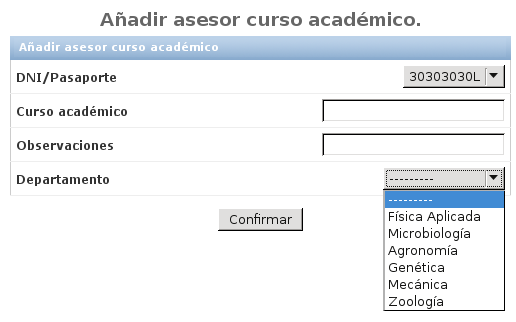
\includegraphics[scale=0.6]{12.Disenyo_Interfaz/12.3.Gestion_Informacion/12.3.2.Adicion_Elementos/adicion_elementos.png}
      }
      \caption{Captura de pantalla de la creación de un nuevo elemento.}
      \label{capturaAdicionElementos}
    \end{center}
  \end{figure}
